\section{Wyniki eksperymentów symulacyjnych}
\begin{frame}
\frametitle{\secname}
\framesubtitle{Otwarta przestrzeń ustawienie prostopadłe}
	\begin{figure}[ht] % h:here; t:top; b:bottom; p:page; default:ht
		\centering
			\captionsetup[subfigure]{labelformat=empty}
			\centering
			\subfloat[][1-2]
			{
				\includegraphics[page = 2, width=0.49\textwidth]{img/Simulation_Open_space.pdf}
			}
			\subfloat[][10-9]
			{
				\includegraphics[page = 99, width=0.49\textwidth]{img/Simulation_Open_space.pdf}
			}
\end{figure}

\note{
\begin{itemize}
	\item Dla ustawienie 1-2 najlepszy łączny czas przejazdu robotów uzyskała algorytm PR. Jako drugi poradził sobie z zadaniem algorytm RVO. Algorytmy R+ oraz R osiągnęły podobne rezultaty.

	\item Przy większej liczbie robotów sytuacja znacząco się zmienia. Algorytm R osiągał najlepszy czas jako drugi algorytm R+. Trzecie miejsce to algorytm RVO zaś najgorzej poradziła sobie metoda PR.
\end{itemize}
}

\end{frame}

\section*{Wyniki eksperymentów symulacyjnych -- materiał wideo}
\begin{frame}[plain]
\frametitle{\secname}
\framesubtitle{Otwarta przestrzeń ustawienie prostopadłe 1-2}

\begin{tikzpicture}[remember picture,overlay]
\node[anchor=south west, inner sep=0pt] at (current page.south west) {%
	\includemedia[addresource=mov/RobotSimulationOpenSpace.mp4,
	activate=pageopen,
	transparent,
	flashvars={source=mov/RobotSimulationOpenSpace.mp4},
	width=\paperwidth,
	height=\paperheight]{}{VPlayer.swf}%
};
\end{tikzpicture}
\end{frame}


\section*{Wyniki eksperymentów symulacyjnych}
\begin{frame}
\frametitle{\secname}
\framesubtitle{Przejście przez drzwi}
\begin{figure}[ht] % h:here; t:top; b:bottom; p:page; default:ht
		\captionsetup[subfigure]{labelformat=empty}
		\centering
		\subfloat[][1-H2]
		{
			\includegraphics[page = 2, width=0.49\textwidth]{img/Simulation_Passage_through_the_door.pdf}
		}
		\subfloat[][9-H8]
		{
			\includegraphics[page = 88, width=0.49\textwidth]{img/Simulation_Passage_through_the_door.pdf}
		}
\end{figure}

\note{

\begin{itemize}
	\item Metoda RVO oraz PR nie poradziły sobie zarówno w ustawieniu 1-H2 oraz 9-H8. Roboty wzajemnie zakleszczyły się w przed przejściem.
	
	\item W obu ustawieniach wyraźnie zaznacza się trend iż metoda PF, PF+ jest nieco lepsza niż metoda R, R+
	
	\item Algorytmy R+ oraz PF+ osiągnęły gorsze wyniki niż metody R oraz R+
\end{itemize}

Litera H – oznaczona w którym pomieszczeniu roboty miały wyższe bazowy współczynnik respektu.

}
\end{frame}

\section*{Wyniki eksperymentów symulacyjnych -- materiał wideo}
\begin{frame}[plain]
\frametitle{\secname}
\framesubtitle{Przejście przez drzwi ustawienie 9-H8}

\begin{tikzpicture}[remember picture,overlay]
\node[anchor=south west, inner sep=0pt] at (current page.south west) {%
	\includemedia[addresource=mov/RobotSimulationPassagePlace.mp4,
	activate=pageopen,
	transparent,
	flashvars={source=mov/RobotSimulationPassagePlace.mp4},
	width=\paperwidth,
	height=\paperheight]{}{VPlayer.swf}%
};
\end{tikzpicture}
\end{frame}

\section*{Wyniki eksperymentów symulacyjnych}
\begin{frame}
\frametitle{\secname}
\framesubtitle{Wąski korytarz}

\begin{figure}[ht] % h:here; t:top; b:bottom; p:page; default:ht
	\captionsetup[subfigure]{labelformat=empty}
	\centering
	\subfloat[][8-3]
	{
		\includegraphics[page = 73, width=0.6\textwidth]{img/Simulation_A_narrow_corridor.pdf}
	}
\end{figure}

\note{
	
	\begin{itemize}
		\item Również i w wąskim korytarzu metody RVO i PR nie poradziły sobie z zadaniem.
		\item Metoda R osiągnęła znacznie lepszy czas przejazdu niż metoda R+
	\end{itemize}
}

\end{frame}

\section*{Wyniki eksperymentów symulacyjnych -- materiał wideo}
\begin{frame}[plain]
\frametitle{\secname}
\framesubtitle{Wąski korytarz ustawienie 8-3}

\begin{tikzpicture}[remember picture,overlay]
\node[anchor=south west, inner sep=0pt] at (current page.south west) {%
	\includemedia[addresource=mov/RobotSimulationNerrowCorridor.mp4,
	activate=pageopen,
	transparent,
	flashvars={source=mov/RobotSimulationNerrowCorridor.mp4},
	width=\paperwidth,
	height=\paperheight]{}{VPlayer.swf}%
};
\end{tikzpicture}
\end{frame}

\section*{Eksperyment na rzeczywistych robotach}
\begin{frame}
\frametitle{\secname}

\begin{itemize}
	\item Obudowa A4WD1v2 Lynxmotion 22cm x 20cm x 6cm.
	\item Zasilanie dwie baterie litowo-polimerowe o nominalnym napięciu 14.8V i pojemności 5Ah.
	\item Sterowniki silników RoboClaw 2 x 15A firmy BasicMicro.
	\item Komputer sterujący PandaBoard ES:	
	\begin{itemize}
		\item dwurdzeniowy procesor Cortex-A9 OMAP4460 taktowany zegarem 1,2 GHz,
		\item RAM 1GB,
		\item Ethernet RJ45 100Mb,
		\item WiFi 802.11 b/g/n i Bluetooth 2.1,
		\item USB 2.0,
		\item I2C,
		\item SPI.
	\end{itemize}
	\item Skaner laserowy URG-04LX-UG01 firmy Hokuyo.	
\end{itemize}

\begin{textblock*}{4cm}(8.5cm,5.2cm) % {block width} (coords)
	\includegraphics[page=1,width=4cm]{img/Rysunki.pdf}
\end{textblock*}
\tiny{
	Open Source Hardware \\
	Strona projektu: \url{http://capo.iisg.agh.edu.pl/}}

\note{
W celu zweryfikowania poprawności działania algorytmów wykorzystano Czterokołową Autonomiczną Platformę Mobilną CAPO zbudowaną na AGH.

Platforma:

\begin{itemize}
	\item zasilana jest z dwóch baterii litowo-polimerowych, 
	\item napędzane jest przez 4 silniki kontrolowane przez dwa kontrolery RoboClaw 2 x 15A firmy BasicMicro,
	\item które kontroluje komputer sterujący PandaBoard ES.
\end{itemize}

Platforma może być dowolnie konfigurowana. Na rysunku widzimy robota CAPO z zaistalowanym skanerem laserowym firmy Hokuyo.

}
\end{frame}

\section{Wyniki eksperymentów z wykorzystaniem rzeczywistych robotów}
\begin{frame}
\frametitle{\secname}
\framesubtitle{Otwarta przestrzeń ustawienie prostopadłe}
\begin{figure}[ht] % h:here; t:top; b:bottom; p:page; default:ht
	\captionsetup[subfigure]{labelformat=empty}
	\centering
	\subfloat[][1-2]
	{
		\includegraphics[page = 2, width=0.6\textwidth]{img/Robots_Open_space.pdf}
	}
\end{figure}

\note{
\begin{itemize}
	\item Najlepiej z przejazdem poradziła sobie metoda PR.
	\item Metody R oraz R+ osiągnęły podobny rezultat.
	\item Metoda RVO zakończyła swoje działanie jako ostatnia.
\end{itemize}

}

\end{frame}


\section*{Wyniki eksperymentów z wykorzystaniem rzeczywistych robotów -- materiał wideo}
\begin{frame}[plain]
\frametitle{\secname}
\framesubtitle{Otwarta przestrzeń ustawienie prostopadłe 1-2}

\begin{tikzpicture}[remember picture,overlay]
\node[anchor=south west, inner sep=0pt] at (current page.south west) {%
	\includemedia[addresource=mov/RobotRobotOpenSpace.mp4,
	activate=pageopen,
	transparent,
	flashvars={source=mov/RobotRobotOpenSpace.mp4},
	width=\paperwidth,
	height=\paperheight]{}{VPlayer.swf}%
};
\end{tikzpicture}
\end{frame}


\section*{Wyniki eksperymentów z wykorzystaniem  rzeczywistych robotów}
\begin{frame}
\frametitle{\secname}
\framesubtitle{Przejście przez drzwi}
\begin{figure}[ht] % h:here; t:top; b:bottom; p:page; default:ht
	\captionsetup[subfigure]{labelformat=empty}
	\centering
	\subfloat[][1-H2]
	{
		\includegraphics[page = 2, width=0.6\textwidth]{img/Robots_Passage_through_the_door.pdf}
	}
\end{figure}

\note{
\begin{itemize}
	\item Metody RVO oraz PR ze względu na brak rezultatów w symulacji nie były uruchamiana na rzeczywistych robotach.
	\item Najlepiej poradziła sobie metoda PF+ oraz PF.
	\item Algorytm R osiągnął trzeci wynik.
	\item Najgorzej z zadaniem poradziła sobie metoda R+.
\end{itemize}
	
}

\end{frame}

\section*{Wyniki eksperymentów z wykorzystaniem rzeczywistych robotów -- materiał wideo}
\begin{frame}[plain]
\frametitle{\secname}
\framesubtitle{Przejście przez drzwi 1-H2}

\begin{tikzpicture}[remember picture,overlay]
\node[anchor=south west, inner sep=0pt] at (current page.south west) {%
	\includemedia[addresource=mov/RobotRobotPassagePlace.mp4,
	activate=pageopen,
	transparent,
	flashvars={source=mov/RobotRobotPassagePlace.mp4},
	width=\paperwidth,
	height=\paperheight]{}{VPlayer.swf}%
};
\end{tikzpicture}
\end{frame}
